\section{Příklad 4}
% Jako parametr zadejte skupinu (A-H)
\ctvrtyZadani{E}



\bigskip
\centerline{\Large{Poďme rátať!}}
\centerline{Pripravme si základné výpočty:}
\bigskip

\centering
\scalebox{1.5}{$\omega = 2 \times \pi \times f = 180\pi\hspace{2em}$}
\scalebox{1.5}{$Z_{L_1} = j \times \omega \times L_1 = j\times180\pi\times130=\num{23400}j\pi\Omega\hspace{2em}$}
\scalebox{1.5}{$Z_{L_2} = j \times \omega \times L_2 = j\times180\pi\times60 = \num{10800}j\pi\Omega\hspace{2em}$}
\scalebox{1.5}{$Z_{C_1} = - \frac{j}{\omega \times C_1} = \frac{j}{180\pi\times100}=\frac{j}{\num{18000}\pi}\Omega\hspace{2em}$}
\scalebox{1.5}{$Z_{C_2} = - \frac{j}{\omega \times C_2} = \frac{j}{180\pi\times65} = \frac{j}{\num{11700}\pi}\Omega$}
\\
\bigskip
\centerline{Poďme zostaviť matice:}
\centering
\[
\begin{pmatrix}

R_2 + R_1 + Z_{C_1} + Z_{L_1} & - Z_{C_1} - R_1 & - R_2\\
- R_1 - Z_{C_1} & Z_{C_1} + R_1 + Z_{L_2} & -Z_{L_2}\\
- R_2 & - Z_{L_2} & Z_{L_2} + R_2 + Z_{C_2}

\end{pmatrix}^{-1}
\begin{pmatrix}
    0\\
    U_1\\
    -U_2
\end{pmatrix}
=
\begin{pmatrix}
    I_a\\
    I_b\\
    I_c
\end{pmatrix}
\]\\
\bigskip

\centerline{Čas na dosadenie:}
\centering
\[
\begin{pmatrix}
    14+13+\frac{j}{\num{18000}\pi}+\num{23400}j\pi &-\frac{j}{\num{18000}\pi}-14 &-13\\
    -14-\frac{j}{\num{18000}\pi} &\frac{j}{\num{18000}\pi}+14+\num{10800}j\pi&-\num{10800}j\pi\\
    -13 &-\num{10800}j\pi &\num{10800}j\pi+13+\frac{j}{\num{11700}\pi}
    
\end{pmatrix}^{-1}
\begin{pmatrix}
    0\\
    5\\
    -3
\end{pmatrix}
=
\begin{pmatrix}
    I_a\\
    I_b\\
    I_c
\end{pmatrix}
\]\\
\bigskip
\newpage
\centerline{Inverzia tejto matice je ťažká. Priložím jej obrázok ale s výpočtami budeme pokračovať až pre napätia.}
\centering
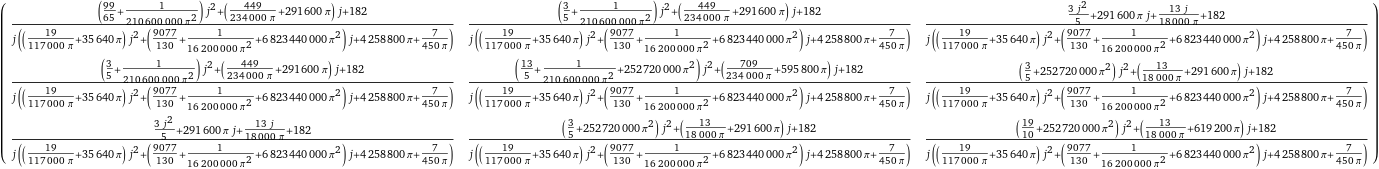
\includegraphics[width=\textwidth,height=\textheight,keepaspectratio]{fig/inverzia.png}
\\
\bigskip
\centerline{Po inverzii a vynásobení týchto matíc nám vyjde matica o rozmeroch 1$\times$3}
\bigskip
\centering
\scalebox{1.5}{$I_a = -0.007 + 0.0126j A\hspace{2em}$}
\scalebox{1.5}{$I_b = 0.0326 - 0.0625j A\hspace{2em}$}
\scalebox{1.5}{$I_c = -0.019 + 0.1077j A$}
\\
\bigskip
\centerline{Poďme to dotiahnuť do konca:}
\bigskip
\centering
\scalebox{1.1}{$ U_{L_2} = \lvert Z_{L_2} \times (I_b - I_c) \rvert = \num{10800}j\pi\times((0.0326-0.0625j)-(-0.019+0.1077j))\approx \underline{\underline{6.0334V}}$}
\\
\bigskip
\centering
\scalebox{1.49}{$\varphi=atan(\frac{\text{imaginárna zložka }U_{L_2}}{\text{reálna zložka }U_{L_2}})\times\frac{180}{\pi}=atan(\frac{1.7535}{5.773})\times\frac{180}{\pi}\approx \underline{\underline{16.8957^{\circ}}}$}


